\documentclass[a4paper, 11pt]{article}

\usepackage[left=2cm, right=2cm, top=2cm, bottom=2cm]{geometry}

\usepackage[utf8]{inputenc} 
\usepackage[T1]{fontenc}      
\usepackage[french,english]{babel}  
\usepackage{lmodern}

\usepackage{amsmath, mathtools}
\usepackage{amssymb}
\usepackage{amsthm}
\usepackage{empheq}
\usepackage{stmaryrd}
\usepackage{upgreek}

\usepackage{graphicx}
\usepackage{subfig}

\usepackage{listings}
\usepackage{color} %red, green, blue, yellow, cyan, magenta, black, white
\definecolor{mygreen}{RGB}{28,172,0} % color values Red, Green, Blue
\definecolor{mylilas}{RGB}{170,55,241}

\usepackage{mathtools}
\DeclarePairedDelimiter\ceil{\lceil}{\rceil}

\lstset{language=Matlab,%
    %basicstyle=\color{red},
    breaklines=true,%
    morekeywords={matlab2tikz},
    keywordstyle=\color{blue},%
    morekeywords=[2]{1}, keywordstyle=[2]{\color{black}},
    identifierstyle=\color{black},%
    stringstyle=\color{mylilas},
    commentstyle=\color{mygreen},%
    showstringspaces=false,%without this there will be a symbol in the places where there is a space
    numbers=left,%
    numberstyle={\tiny \color{black}},% size of the numbers
    numbersep=9pt, % this defines how far the numbers are from the text
    emph=[1]{for,end,break},emphstyle=[1]\color{red}, %some words to emphasise
    %emph=[2]{word1,word2}, emphstyle=[2]{style},    
}

\begin{document}
\title{Rendu TP5 Imagerie sous-pixellique}
\author{Yoann Pradat}
\maketitle

\paragraph{Exercice 13}

\textbf{1.} $u: \mathbb{Z} \to \mathbb{R}$ est un signal. La translation de facteur $\frac{1}{2}$ par interpolation
linéaire est 

\begin{equation}
  \forall k \in \mathbb{Z} \quad v[k] = \frac{1}{2}(u[k-1] + u[k])
\end{equation}

On en déduit

\begin{align*}
  \forall \xi \in \mathbb{R} \quad \hat{v}(\xi) &= \frac{1}{2} ( \sum_{k \in \mathbb{Z}} u[k-1] e^{-ik\xi} + \hat{u}(\xi))\\
  &= \frac{1}{2}\hat{u}(\xi) (e^{-i\xi} + 1) \\
  &= \hat{u}(\xi) e^{\frac{-i\xi}{2}} \cos(\frac{\xi}{2}) 
\end{align*}

Regardons désormais le lien entre transformée de Fourier de l'interpolée de Shannon et transformée de Fourier de $u$.
L'interpolée de Shannon est 

\begin{equation}
  \forall x \in \mathbb{R} \quad U(x) = \sum_{k \in \mathbb{Z}} u[k] \text{sinc}(x-k)
\end{equation}

Interpoler revient à restreindre la transformée de Fourier de $u$ à $[-\pi, \pi]$ et $\hat{u}$ et $\hat{U}$ coïncident
sur $[-\pi, \pi]$ d'où

\begin{equation*}
  \forall x \in \mathbb{R} \quad U(x) = \frac{1}{2\pi} \int_{-\pi}^{\pi} \hat{u}(\xi) e^{ix\xi} d\xi
\end{equation*}

Alors $\displaystyle U(k-\frac{1}{2}) =  \frac{1}{2\pi} \int_{-\pi}^{\pi} \hat{u}(\xi) e^{-i\frac{\xi}{2}} e^{ik\xi}
d\xi$ mais aussi  $\displaystyle w[k] = \frac{1}{2\pi} \int_{-\pi}^{\pi} \hat{w}(\xi) e^{ik\xi} d\xi$ et évidemment $w[k] =
U(k-\frac{1}{2})$. Par unicité de la transformée de Fourier on en déduit $\hat{w}(\xi) = \hat{u}(\xi)
e^{\frac{-i\xi}{2}}$. \\

On en déduit finalement le lien souhaité \fbox{$\hat{v}(\xi) = \hat{w}(\xi) \cos(\frac{\xi}{2})$}. \\

\textbf{2.} L'interpolation linéaire entre $u[k]$ et $u[k+1]$ est $v(x) = (k+1-x)u[k] + (x-k)u[k+1]$. Pour obtenir un
zoom de facteur 2 il suffit d'intercaler un nouveau pixel entre chaque paire de pixels par interpolation linéaire de sorte 
que le signal zoomé $v$ est donné par

$$ \forall k \in \mathbb{Z}  \quad \left\lbrace
\begin{array}{lll}
  v[2k]&=& u[k] \\
  v[2k+1]&=& \frac{1}{2}(u[k] + u[k+1])
\end{array}
\right.$$

\clearpage

Alors 

\begin{align*}
  \forall \xi \in \mathbb{R} \quad  \hat{v}(\xi) &= \sum_{k \in \mathbb{Z}} v[k] e^{-ik\xi} \\ 
  &= \sum_{k \in \mathbb{Z}} v[2k] e^{-i2k\xi} + \sum_{k \in \mathbb{Z}} v[2k+1] e^{-2ik\xi - i\xi} \\
  &= \hat{u}(2\xi) + \frac{1}{2} \left( \sum_{k \in \mathbb{Z}} u[k] e^{-2ik\xi} + \sum_{k \in \mathbb{Z}} u[k+1]
e^{-2ik\xi} \right) \\
  &= \hat{u}(2\xi) + \frac{\hat{u}(2\xi)}{2} e^{-i\xi} ( 1 + e^{2i\xi}) \\
  &= \hat{u}(2\xi) (1+\cos(\xi))
\end{align*}

On regarde désormais le zoom de facteur 2 obtenu par interpolation de Shannon $w$. En reprenant l'expression dans la question 
\textbf{1.} de l'interpolée de Shannon $U$ en fonction de $\hat{u}$ on a

\begin{align*}
  \forall k \in \mathbb{Z} \quad w[k] &= U(\frac{k}{2}) \\
  &= \frac{1}{2\pi} \int_{-\pi}^{\pi} \hat{u}(\xi) e^{i\frac{k}{2}\xi} d\xi \\
  &= \frac{1}{2\pi} \int_{-\frac{\pi}{2}}^{\frac{\pi}{2}} 2\hat{u}(2\xi) e^{ik\xi} d\xi \\
  &= \frac{1}{2\pi} \int_{-\pi}^{\pi} \hat{w}(\xi) e^{ik\xi} d\xi
\end{align*}

A nouveau par unicité de la transformée de Fourier on obtient

$$ \forall \xi \in [-\pi, \pi]  \quad  \hat{w}(\xi)=\left\lbrace
\begin{array}{lll}
  &2\hat{u}(2\xi) \quad &\text{si } \xi \in [-\frac{\pi}{2}, \frac{\pi}{2}] \\
  &0 \quad &\text{sinon} 
\end{array}
\right.$$

et $\hat{w}$ est étendue sur $\mathbb{R}$ par $2\pi$-périodisation. Ainsi,


$$\boxed{ \forall \xi \in [-\pi, \pi]  \quad  \hat{v}(\xi)=\left\lbrace
\begin{array}{llll}
  &\hat{w}(\xi) \cos^2(\frac{\xi}{2}) \quad &\text{si } \xi \in &[-\frac{\pi}{2}, \frac{\pi}{2}] \\
  &\hat{w}(\xi-\pi) \cos^2(\frac{\xi}{2})  \quad &\text{si } \xi \in &]\frac{\pi}{2}, \pi] \\
  &\hat{w}(\xi+\pi) \cos^2(\frac{\xi}{2}) \quad &\text{si } \xi \in &[-\pi, -\frac{\pi}{2}[ \\
\end{array}
\right.}$$

Cette formule est valable sur $\mathbb{R}$ tout entier par $2\pi$-périodisation. \\

\textbf{3.} Désormais le signal est $u: \Omega \to \mathbb{R}$. Dans ce cas l'interpolation de Shannon de $u$ est 

\begin{equation}
  U(x,y) = \frac{1}{MN} \sum_{|p| \leq \frac{M}{2}, |q| \leq \frac{N}{2}} \epsilon_M(p) \epsilon_N(q) \hat{u}[p,q]
  e^{\frac{2i\pi px}{M} + \frac{2i\pi qy}{N}}
\end{equation}

Le zoom de facteur 2 est obtenu par la transformation $U(\frac{x}{2}, \frac{y}{2})$ d'où

\begin{equation*}
  w(x,y) = \frac{1}{MN} \sum_{|p| \leq \frac{M}{2}, |q| \leq \frac{N}{2}} \epsilon_M(p) \epsilon_N(q) \hat{u}[p,q]
  e^{\frac{2i\pi px}{2M} + \frac{2i\pi qy}{2N}}
\end{equation*}

On peut également former l'interpolée de Shannon de l'image zoomée

\begin{equation*}
  w(x,y) = \frac{1}{4MN} \sum_{|p| \leq M, |q| \leq N} \epsilon_{2M}(p) \epsilon_{2N}(q) \hat{w}[p,q]
  e^{\frac{2i\pi px}{2M} + \frac{2i\pi qy}{2N}}
\end{equation*}

\clearpage

Cela nous permet de relier les transformées de Fourier de $u$ et $w$ par

$$\boxed{ \forall p,q \text{ with } |p| \leq M, |q| \leq N \quad  \hat{w}[p,q]=\left\lbrace
\begin{array}{lll}
  &4 \epsilon_M(p) \epsilon_N(q) \hat{u}[p,q] \quad &\text{si } |p| \leq \frac{M}{2}, |q| \leq \frac{N}{2}\\
  &0  \quad &\text{sinon}\\
\end{array}
\right.}$$

puis on étend à $\mathbb{Z}\times\mathbb{Z}$ par $(M,N)$ périodicité. \\ 

L'interpolation bilinéaire dans $[u[k, l], u[k+1, l]]\times[u[k, l], u[k, l+1]]$ est $v(x, l) = (k+1-x)u[k,l] +
(x-k)u[k+1,l]$ puis $v(x,y) = v(x,l)(l+1-y) + v(x, l+1)(y-l)$ c'est-à-dire

\begin{equation*}
  v(x,y) = (k+1-x)(l+1-y)u[k,l] +(x-k)(l+1-y)u[k+1,l] + (k+1-x)(y-l)u[k,l+1] + (x-k)(y-l)u[k+1,l+1]
\end{equation*}

Pour obtenir un zoom de facteur 2 il suffit d'intercaler un nouveau pixel dans chaque carré de pixels par interpolation
bilinéaire de sorte que le signal zoomé $v$ est donné par

$$ \forall k,l \in \llbracket0, M-1\rrbracket\times\llbracket0, \dots, N-1\rrbracket \quad \left\lbrace
\begin{array}{lll}
  v[2k, 2l]&=& u[k,l] \\
  v[2k+1, 2l]&=& \frac{1}{2}(u[k, l] + \dot{u}[k+1, l]) \\
  v[2k, 2l+1]&=& \frac{1}{2}(u[k, l] + \dot{u}[k, l+1]) \\
  v[2k+1, 2l+1]&=& \frac{1}{4}(u[k, l] + \dot{u}[k, l+1] + \dot{u}[k+1,l] + \dot{u}[k+1, l+1]) \\
\end{array}
\right.$$

On en déduit la transformée de Fourier du signal zoomé $v$

\begin{align*}
  \forall p,q \in \mathbb{Z}\times\mathbb{Z} \quad \hat{v}[p,q] &= \frac{1}{4MN} \sum_{k=0}^{2M-1} \sum_{l=0}^{2N-1} v[k,l] 
  e^{-\frac{2i\pi pk}{2M} - \frac{2i\pi ql}{2N}} \\
  &= \frac{1}{4} \hat{u}[p,q] + \frac{1}{8}\hat{u}[p,q](e^{-\frac{i\pi q}{N}} + e^{\frac{i\pi q}{N}} + e^{-\frac{i\pi p}{M}} + e^{\frac{i\pi p}{M}}) \\
  &\phantom{{}=} + \frac{1}{16}\hat{u}[p,q](e^{\frac{-i\pi p}{M}}e^{\frac{-i\pi q}{N}} + e^{\frac{-i\pi
    p}{M}}e^{\frac{i\pi q}{N}} +  e^{\frac{i\pi p}{M}}e^{\frac{-i\pi q}{N}} +  e^{\frac{i\pi p}{M}}e^{\frac{i\pi q}{N}})  
\end{align*}

c'est-à-dire

\begin{equation*}
  \boxed{\forall p,q \in \mathbb{Z}\times\mathbb{Z} \quad \hat{v}[p,q] = \frac{1}{4} \hat{u}[p,q] \left(1 + \cos(\frac{\pi p}{M}) + \cos(\frac{\pi q}{N}) +  
    \cos(\frac{\pi p}{M})\cos(\frac{\pi q}{N}) \right)}
\end{equation*}

On peut maintenant faire le lien entre $\hat{w}$ et $\hat{v}$ mais c'est assez fastidieux à écrire.

\paragraph{Exercice 3}

\textbf{1.} On note $\alpha$ l'angle (en radians) sous lequel Saturne est vue par le télescope. On note $f$ la focale du
télescope et $x$ le diamètre de l'image de Saturne sur le plan focal image. Clairement $x = f\tan(\alpha)$. A
l'échantillonnage critique correspondant à la limite spectrale de la diffraction les pixels sont de taille exactement
$\delta_c$ avec $\delta_c = \frac{\lambda f}{2D}$ où $\lambda$ est la longueur d'onde des rayons dont on forme l'image.
Pour l'application numérique on prend pour $\lambda$ le centre du spectre visible soit $6\times 10^{-7}$ m. \\

Le nombre recherché est le diamètre $x$ de l'image sur la taille d'un pixel $\delta_c$ soit 

\begin{align*}
  N &= \frac{\tan(\alpha)f}{\frac{\lambda f}{2D}}  \\
  &= \frac{2D\tan(\alpha)}{\lambda} \\
  &\approx 30 \text{ pixels} 
\end{align*}

\clearpage

\textbf{2.} Cette fois l'objet observé est un pixel, le plan focal est la rétine et la lentille est la
pupille de l'œil. On note toujours $\alpha$ l'angle sous lequel le pixel est vu, $d$ la distance du pixel à l'oeil, $x$
la taille de l'image du pixel formée sur la rétine, $f$ la focale de la pupille et $c$ la taille d'un pixel. Alors 

\begin{equation*}
  \tan(\alpha) = \frac{c}{d} = \frac{x}{f}
\end{equation*}

On ne distingue plus les pixels à partir du moment où les taches de diffractions de deux pixels contigus ne sont plus
discernables sur notre rétine. D'après le TP1 cela se produit lorsque les centres de ces deux taches de diffraction sont
distants d'environ 77\% du rayon d'Airy $r_a = 1.22\frac{\lambda f}{D}$. On a donc à la distance critique  

\begin{equation*}
  x = 0.77\times1.22\frac{\lambda f}{D} \implies d = \frac{0.77\times1.22Dc}{\lambda} 
\end{equation*}

Application numérique: D = 0.005 m, c = $\frac{0.5}{1080}$ d'où d $\approx$ 3.6 m \\

\textbf{3.} On a vu en cours que la diffraction crée des images à bande limitée avec coupure critique
$\frac{\pi}{\delta_c}$. Échantillonner avec un pas de $\delta_c = \frac{\lambda f}{2D}$ est donc le pas critique pour un
bon échantillonnage (pas d'aliasing) alors qu'un pas $\delta < \delta_c$ produit un sur-échantillonnage et inversement
$\delta > \delta_c$ un sous-échantillonnage par rapport aux effets de la diffraction. On note $c$ la taille d'un pixel 
(longueur d'un côté du carré). Pour un appareil 24 mm $\times$ 36 mm avec 30 Mpixels la taille $c$ est donnée par $c =
\sqrt{\frac{0.026\times0.036}{30\times10^6}} = 5.6 \upmu\text{m}$. \\

Prenons les hautes fréquences du spectre visible i.e $\lambda = 0.4 \upmu\text{m}$. Alors on est en sur-échantillonnage
tant que $\frac{\lambda f}{2D} > c$ i.e $\frac{f}{D} > \frac{2c}{\lambda} = 28$. 

Pour les basses fréquences du spectre visible i.e $\lambda = 0.8 \upmu\text{m}$, on est en sur-échantillonnage
tant que $\frac{f}{D} > \frac{2c}{\lambda} = 14$. \\ 

\paragraph{Exercice 16} On applique une translation sous-pixellique de vecteur ($\frac{1}{2}$,$\frac{1}{2}$) à l'image
“bouc.pgm” et on forme la différence entre l'image et sa translatée pour obtenir

\begin{figure}[!h]
  \centering
  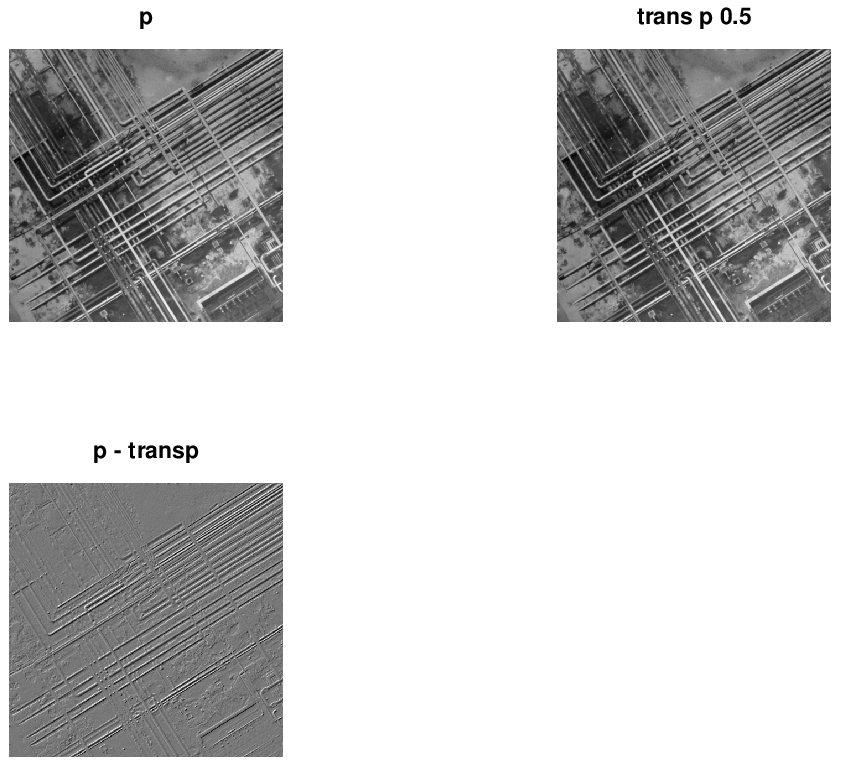
\includegraphics[width=10cm]{bouc_p_ffttrans.png}
  \caption{Translatée d'un demi-pixel}
  \label{fig:bouc_0.5}
\end{figure}

Le résultat est celui escompté mais on observe toutefois l'apparition de discontinuités dans les bords gauche et haut de
l'image translatée. Accentuons la translation à (50.5, 50.5) pixels pour bien observer ce qui se passe.

\begin{figure}[!h]
  \centering
  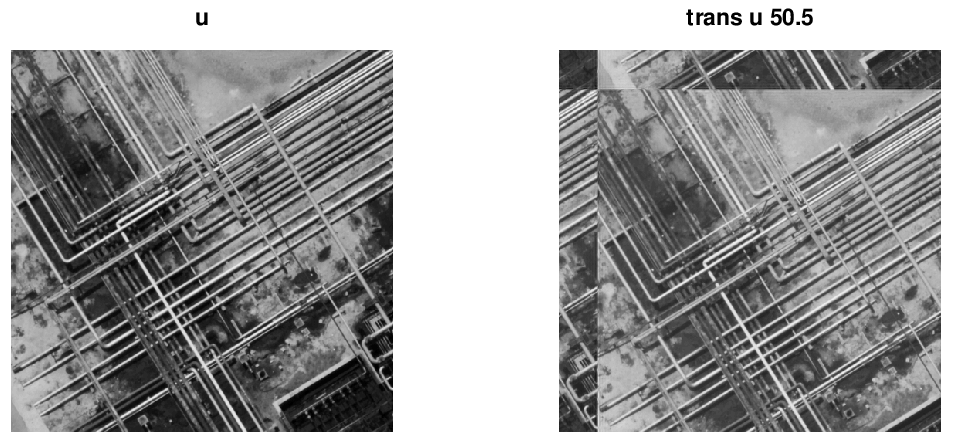
\includegraphics[width=10cm]{bouc_p_ffttrans_50.png}
  \hfill
  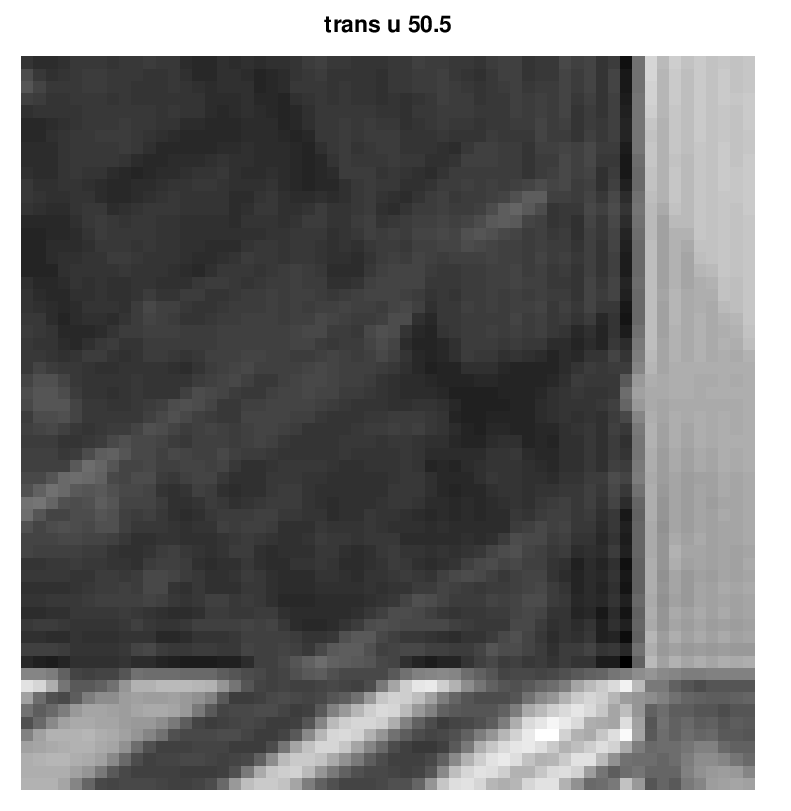
\includegraphics[width=4.5cm]{ringing_50.png}
  \caption{Translatée de 50.5 pixels et zoom sur ringing}
  \label{fig:bouc_50.5}
\end{figure}

On voit clairement dans le cadran droit supérieur sur l'image zoomée un effet de \textbf{ringing} à la jonction entre l'image
originale et la translation. \\

On peut envisager une décomposition périodique + \og smooth \fg et ne translater que la partie périodique par exemple:
cela correspond à l'image de droite sur la figure~\ref{fig:bouc_transp_s}.

\begin{figure}[!h]
  \centering
  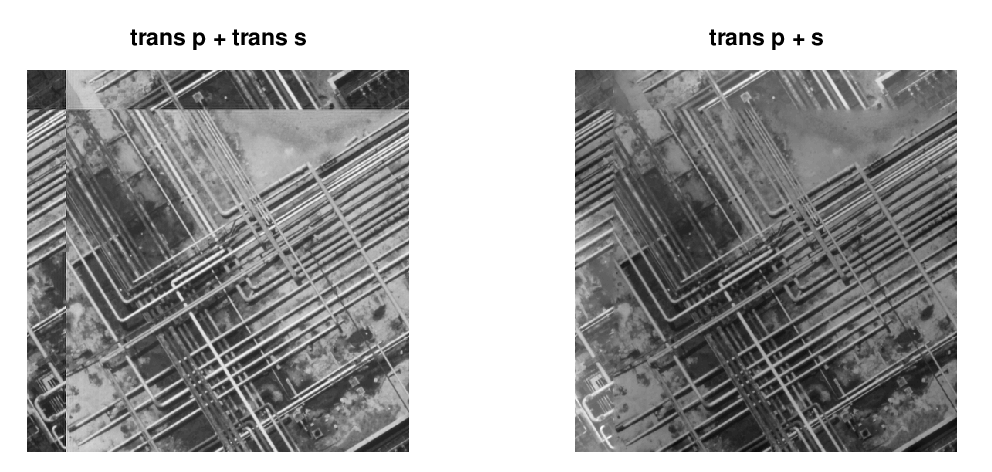
\includegraphics[width=8cm]{bouc_perdecomp_trans_50.png}
  \caption{Translatée de 50.5 pixels et décomposition \texttt{p+s}}
  \label{fig:bouc_transp_s}
\end{figure}


Il n'y a plus d'effets de ringing mais les niveaux de gris sont complètement faux comparés à ceux de l'image originale.
Il faut donc translater la partie smooth aussi. Toutefois translater les la partie périodique et la partie smooth du
même vecteur (50.5, 50.5) fait la même chose que translater \texttt{u} et donc produit du ringing. On peut envisager
plutôt de translater \texttt{s} non pas de (50.5, 50.5) mais de (50, 50) et observe ce qui se passe. Cela correspond à
la figure ~\ref{fig:bouc_trans_round} ci-dessous. Avec une translation de la partie \og smooth \fg du vecteur d'entiers le
plus proche le ringing a complètement disparu !

\begin{figure}[!h]
  \centering
  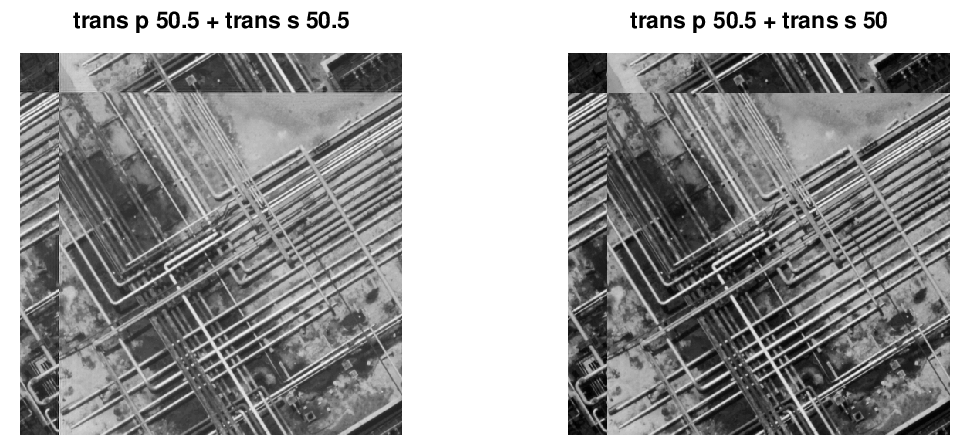
\includegraphics[width=8cm]{bouc_perdecomp_trans_50_round.png}
  \hfill
  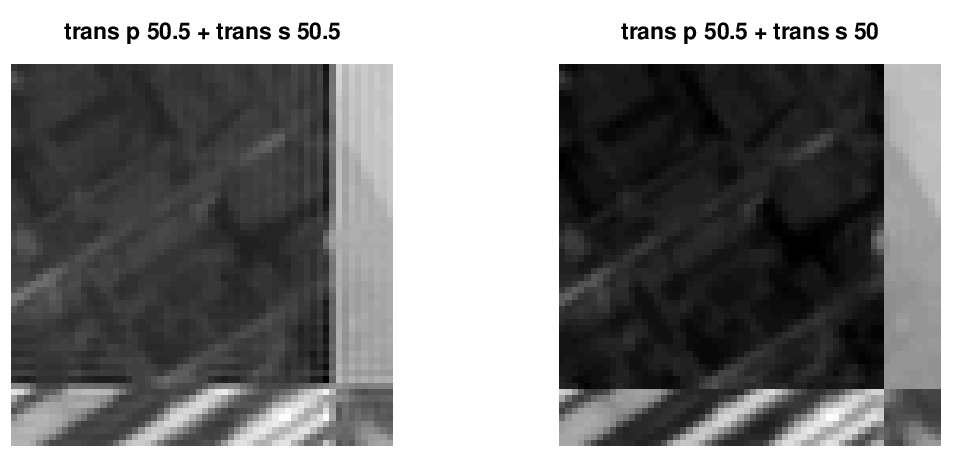
\includegraphics[width=8cm]{bouc_perdecomp_trans_50_round_zoom.png}
  \caption{(g) Translatée de 50.5 \texttt{p} et \texttt{s},  translatée de 50.5 \texttt{p} et de 50 \texttt{s} (d) idem
  mais zoom}
  \label{fig:bouc_trans_round}
\end{figure}

\end{document}



